\chapter{Theoretical Background}
\label{chap:background_RL}

\begin{comment}
Background
Fundamentals - MDPs, ValueFunctions
Policy Gradient Methods - Actor-Critc
DDPG
PPO

\begin{itemize}
    \item drone dynamics
    \item MDPs
    \item RL in the continous domain
    \item Policy gradient methods
    \item DDPG
    \item PPO
\end{itemize}
\end{comment}

\section{Overview}

In this section, we will cover the necessary theoretical background required to understand DDPG and PPO. This will start with a gentle introduction to basic RL concepts, including Markov Decision Processes and returns, before moving on to policies and value functions. 

To get an overview of the basics of reinforcement learning, we can begin by looking into its definition and goal. Sutton and Barto \cite{suttonAndBartoBook} states, ``reinforcement learning is learning what to do -- how to map situations to actions -- so as to maximise a numerical reward signal.''
Also, \cite{RLinRoboticsSurvey} states that ``reinforcement learning enables a robot to autonomously discover an optimal behavior through trial-and-error interactions with its environment."

From these, we note a few terms that are worthy of an explanation, such as \textit{situations, actions, rewards, behaviour, trial-and-error interactions} and \textit{environment}.
We can also ask ourselves, ``what exactly is an \textit{optimal} behaviour and how to we express this?''

These concepts are central to reinforcement learning and by the end of this chapter these should be understood. This brings us to the first section, where we will look into Markov Decision Processes.

\section{Finite Markov Decision Processes}
\label{sec:MDPs}

Finite Markov Decision Processes (MDPs) are essentially a standardised learning framework for reinforcement learning. Formally, the MDP framework is comprised of a few elements, often depicted in a diagram as shown in Figure \ref{fig:2_1_simpleMDP}. This diagram depicts an iterative loop: starting first with an initial state, taking an action, observing a new state and reward, then taking the next action and so on.
\begin{figure}[hbt]
    \centering
    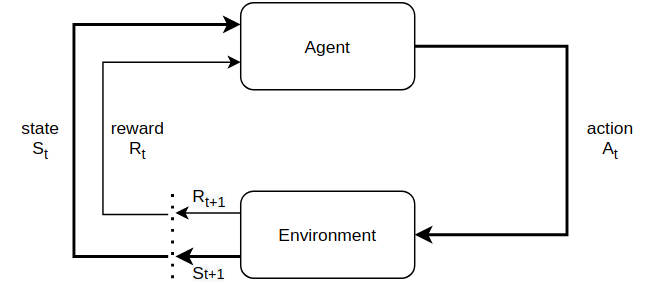
\includegraphics[width=0.8\textwidth]{figures/2_/2_1_simpleEnv2.png}
    \caption{The interaction between agent and environment in an MDP$ $, from \cite{suttonAndBartoBook}.}
    \label{fig:2_1_simpleMDP}
\end{figure}

The first element of an MDP is the \textit{agent}. The agent has the task of \textit{learning} how to solve a specific goal, whereby continuously trying to improve their performance through experience -- or interactions with the \textit{environment}. The \textit{environment} can be thought of as the controlled system, while the agent as the controller.
The situations that an agent finds itself in is referred to as \textit{states} or \textit{observations}. Every state also has the Markov Property, which requires the information in that state only to be dependent on the previous state $S_{t-1}$ and action $A_t$ \cite{suttonAndBartoBook}. 
From a state $S_{t} \in \mathcal{S}$, the agent can take an \textit{action} $A_{t}\in \mathcal{A}$, where $\mathcal{S}$ is the set of states possible and $\mathcal{A}$ is a set of actions for $S_{t}$.
Actions in this case are comparable to control signals and can refer to anything that transitions an agent into a new state such as the acceleration input to a quadrotor or individual torques to rotors. 

An MDP is also includes a \textit{state distribution} $p(s)$ and the states the agent moves to is based on the \textit{state-transition dynamics} $p(s',r|s, a)$, a deterministic function with four arguments that captures the dynamics of the MDP and describes the probability of a specific transition \cite{suttonAndBartoBook}:
\begin{equation}
    p\hspace{0.5mm} (s',r \hspace{0.5mm}|\hspace{0.5mm} s, a) = P \hspace{0.5mm} (S_t = s', \hspace{0.5mm}R_t = r \hspace{0.5mm}|\hspace{0.5mm} S_{t-1} = s,\hspace{0.5mm} A_{t-1} = a )
\end{equation}
Note that $S_t$, $R_t$ and $A_t$ are random variables with well defined probability distributions, while $s$, $r$ and $a$ are particular values of these random variables. The value $s'$ is often a common choice to denote the value of the next state from $s$.

As we can see, the agent receives a numerical \textit{reward} $R_t \in \mathcal{R} \subset \mathbb{R}$ directly from the environment when entering a state $S_t$, which is a sort of evaluative feedback. The reward can be also be function $R(s,a)$ based on the state $s$, action $a$, or also $R(s',a,s)$ which includes the next state $s'$ \cite{TTK23, RLinRoboticsSurvey}. The set $\mathcal{R}$ is used to represent the finite set of rewards possible in an MDP.

To summarise, an MDP can be modelled as the tuple $\langle \mathcal{S},\mathcal{A}, p, R \rangle$, where $\mathcal{S}$ is a finite set of states, $\mathcal{A}$ the finite set of actions for any $S \in \mathcal{S}$, $p$ the state-transition dynamics function $p : \mathcal{S} \times \mathcal{R} \times \mathcal{S} \times \mathcal{A} \rightarrow \mathbb{R} \in [0,1]$  and the reward function $ R : \mathcal{S} \times \mathcal{A} \times \mathcal{S} \rightarrow \mathbb{R}$ \cite{TTK23}.

\section{Returns and Optimal Criteria}
\label{sec:2_ReturnsAndOptimalCriteria}

Now that we have defined MDPs as a framework for learning, we can guess that the agent will try different actions in different states. Eventually, this should allow it to discover an optimal behaviour -- essentially knowing which action is best for each state $s \in \mathcal{S}$. Before, we look into the how to find this behaviour, we will first need to specifically define what we by ``good'' or ``bad'' behaviour.

We start by defining the goal of reinforcement learning. As mentioned at the beginning of the chapter, the aim of reinforcement learning is informally, ``to maximise a numerical reward signal''. The reward signal in this case is a scalar, received every time step at each new state and serves as an immediate feedback for the action the agent took. Yet, if we consider the formulation of MDPs more carefully, taking a certain action a particular state does not only affect the state the agent transitions to in the next time step, but also affects all consequent states and rewards for all following time steps. This illustrates the concept of \textit{delayed reward}, which suggests that receiving a high reward now does not necessarily mean receiving a high reward later.

Therefore, it is important to define the goal of reinforcement learning in the context of reward more precisely. As such, we define the \textit{return} $G_t$, as a specific function of a sequence of rewards $R_t, R_{t+1}, R_{t+2}, ...$. For example, the simplest return can be defined as the sum of a sequence of rewards:
\begin{equation}
    G_t = R_t + R_{t+1} + R_{t+1} + ... + R_{T}
\end{equation}
The idea of a return allows us to then define an optimality criteria where the objective is to maximise the \textit{expected} return $G_t$ over some time horizon:
\begin{equation}
    J = \E \hspace{0.5mm} [G_t] = \E\hspace{0.5mm}\left[ \sum^{T}_{k=t+1} R_{k} \right]
\end{equation}
Here, $T$ is a random variable that denotes the time of termination, which is often the last timestep of an \textit{episode}. An episode can be understood as a series of timesteps of performing a task and this task ends when we reach a \textit{terminal} state.

However, in the case of robotic control tasks, there is often no clear end-of-episode scenario and the task is rather a never-ending continuing process. For such problems, the time horizon is infinite and the optimality criteria instead shifts to maximising what is referred to as the expected \textit{discounted return} \cite{suttonAndBartoBook}:
\begin{equation}
    J = \E \hspace{0.5mm}[G_t] = \E \hspace{0.5mm} \left[ \sum^\infty_{k=0} \gamma^t R_{t+k+1} \label{eq:2_3_discReturn} \right]
\end{equation}
where $\gamma \in [0,1)$ is referred to as the \textit{discount factor} -- an exponentially decreasing weight on \textit{future rewards} -- chosen normally to be either 0.9 or 0.99. This bound on $\gamma$ also ensures that the infinite sum of rewards is finite, and serves a purpose on determining the behaviour of the agent. If the discount factor $\gamma$ is low, the agent (greedily) prioritises short term rewards over perhaps greater long term rewards, and if $\gamma$ is too low, the optimal control law can be unstable \cite{RLinRoboticsSurvey}. On the contrary, if $\gamma$ is high, the agent will be more farsighted, which can lead to unnecessary actions in the short-term. 

Another interesting property that is important for the concepts and algorithms we introduce later is the recursive expression of returns for successive time steps:
\begin{align}
    G_t &= R_{t+1} + \gamma R_{t+2} + \gamma^2 R_{t+3} + \gamma^3 R_{t+4} ... \nonumber \\
    G_t &= R_{t+1} + \gamma (R_{t+2} + \gamma R_{t+3} + \gamma^2 R_{t+4} ...) \nonumber \\
    G_t &= R_{t+1} + \gamma G_{t+1} \label{Eq:2_1_RecReturns} 
\end{align}

So, with the goal of reinforcement learning defined more clearly in terms of maximising the expected discounted return, we can finally proceed to finding out how an agent can learn an optimal behaviour.

\section{Policies and Value Functions}
\label{sec:2_PoliciesValueFunc}

First, the behaviour that an agent learns is called a \textit{policy} $\pi$. Formally, it is defined as a function mapping of states to probabilities of selecting each possible action, $\pi(s,a) = P(a|s)$ \cite{suttonAndBartoBook}. Despite this, a policy $\pi$ can also be deterministic, resulting in the same action for a state every time, written as $a = \pi(s)$ \cite{RLinRoboticsSurvey}.

Initially, we can imagine that the policy, that governs the actions taken by the agent, could be quite random and non-ideal. Then throughout its learning process, the agent will receive rewards $r$, accumulate returns, and update its policy $\pi$ consequently. So, when we think about an optimal policy $\pi^*$, we imagine an agent performing the actions that results in the best result.
Hence, we can say that in order to solve the reinforcement learning problem, we need to ``solve'' the MDP by finding this optimal policy $\pi^*$. 

The method forward is to define a \textit{state-value function} $V_\pi$, which indirectly tells us how good it is to be in a particular state. For MDPs, the state-value function can be defined as the expected return for being in a state $s$ and following a policy $\pi$ thereafter \cite{suttonAndBartoBook}:
\begin{equation}
    V^\pi(s) = \E_\pi [G_t \hspace{0.5mm} | \hspace{0.5mm} S_t = s] = \E_\pi \left[\sum^\infty_{k=0} \gamma^t R_{t+k+1} \hspace{0.5mm} \Bigg| \hspace{0.5mm} S_t = s \right] \forall s \in \mathcal{S}
\end{equation}
Similarly, we can define an \textit{action-value function} (or \textit{Q-function}), as the expected return for being in a state $s$ and taking an action $a$, and following a policy $\pi$ thereafter \cite{suttonAndBartoBook}:
\begin{equation}
    Q^\pi(s,a) = \E_\pi [G_t \hspace{0.5mm} | \hspace{0.5mm} S_t = s, A_t = a] = \E_\pi \left[\sum^\infty_{k=0} \gamma^t R_{t+k+1} \hspace{0.5mm} \Bigg| \hspace{0.5mm} S_t = s, A_t = a \right]
\end{equation}
In other words, these value functions represent the total reward you can expect by following a policy $\pi$ (e.g. until the end of an episode), from a particular state $s$. Informally, the state-value function is simply referred to as the value function $V(s)$, and is how we refer to it throughout this project. The difference between the value function $V$ and the \textit{Q}-function is that the value function gives the expected return for a state $s$ assuming the agent takes the action $a$ decided by $\pi$, while the \textit{Q}-function evaluates the expected return at a state $s$ based on different choices of actions $a$.

A fundamental property of value functions is that they also possess the recursive property similar to that of returns in \eqref{Eq:2_1_RecReturns}:
\begin{align}
    V^\pi(s) &= \E_\pi [G_t \hspace{0.5mm} | \hspace{0.5mm} S_t = s] \nonumber \\
    &= \E_\pi [R_{t+1} + \gamma G_{t+1} \hspace{0.5mm} | \hspace{0.5mm} S_t = s] \nonumber \\
    &= \sum_a \pi(a|s) \sum_{s'}\sum_r \hspace{0.5mm} p(s', r \hspace{0.5mm}|\hspace{0.5mm} s, a) \hspace{0.5mm} \Big[r + \gamma \E_\pi [G_{t+1} \hspace{0.5mm} | \hspace{0.5mm} S_{t+1} = s'] \Big] \nonumber \\
    &= \sum_a \pi(a|s) \sum_{s',r} p(s', r \hspace{0.5mm}|\hspace{0.5mm} s, a) \hspace{0.5mm} \Big[r + \gamma V^\pi(s') \Big] \label{Eq:2_1_valueFunc}
\end{align}
as shown in \cite{suttonAndBartoBook}. First, we expand according to \eqref{Eq:2_1_RecReturns}. Then, we expand the expectation to $R_{t+1}$ and $G_{t+1}$, and use the definition of the expectation. This yields a sum over the possible actions, next states and rewards for a certain state, where the return for that outcome is weighted with its probability. The weight for each possible outcome is given by the product of the probability of selecting action $a$ given $s$, $\pi(a|s)$, and transitioning to state $s'$, or $ p(s', r \hspace{0.5mm}|\hspace{0.5mm} s, a)$.
Finally, we recognise the value function term for the next timestep to yield \eqref{Eq:2_1_valueFunc}. This equation is often referred to as the \textit{Bellman equation for} $V^\pi$ \cite{BellmanDreyfus1962Book}.

Perhaps easier to read is the formulation of \cite{watkins1992QLearning} (with a slight difference in notation):
\begin{equation}
    V^\pi(s) = R_s(a) + \gamma \sum_{s'} p\big(s', r \hspace{0.5mm}|\hspace{0.5mm} s, a \big) \hspace{1mm} V^\pi(s') \,\, \Big|_{a = \pi(s)}
\end{equation}
which uses the deterministic form of policy, $a = \pi(s)$, which outputs an action $a$ instead of probabilities for actions based on a state $s$. Through this we can see that the value of a state, $V^\pi (s)$, is the immediate reward received for that state, plus the weighted sum of the values of the next possible states, under a policy $\pi$.

With these value and action-value (or Q) functions we can formalise how an agent can know what is ``best''. When in a particular state, the agent now not only has the capability to know how much reward it can expect, but also the expected return for each possible action it can take when in that state.
From this, we can see that a sensible policy would be to simply choose the actions with the highest expected return for every timestep. This greedy solution is actually the correct approach, however it comes with the assumption that our value functions are \textit{optimal}. So, as a result, many learning algorithms for MDPs compute optimal policies by learning value functions \cite{TTK23}.


\section{Optimal Policies and Value Functions}
\label{sec:2_optimalPoliciesValueFunc}

Optimal policies can be defined as a policy $\pi$ whose expected return is greater than or equal to all other policies $\pi' \hspace{1mm} \forall s \in \mathcal{S}$ \cite{suttonAndBartoBook}.
By the theory of \cite{BellmanDreyfus1962Book}, we know that there is at least one optimal value function that follows $\pi^*$. An optimal value function is denoted:
\begin{equation}
    V^{\pi^*}(s) = \max_\pi V^\pi(s)
\end{equation}
while, an optimal Q-function is denoted:
\begin{align*}
    Q^{\pi^*}(s,a) &= \max_a Q^\pi(s,a)
\end{align*}
This optimal Q-function is defined as the expected return of a state $s$ and taking an action $a$, then following the optimal policy thereafter:
\begin{align} 
    Q^{\pi^*}(s,a) &= \max_\pi \hspace{0.5mm} \E \hspace{0.5mm} \big[ R_{t+1} + \gamma \hspace{0.5mm} V^{\pi^*}(S_{t+1}) \hspace{0.5mm} \big| \hspace{0.5mm} S_t = s, \hspace{0.5mm} A_t = a \big]
\end{align}
Going further, we see that the optimal value function is identical to the optimal Q-function when taking the best action:
\begin{align*}
    V^{\pi^*}(s) &= \max_{a \in \mathcal{A}(s)} Q^{\pi^*}(s,a) \numberthis \label{2_5_v*} \\
    &= \max_a \hspace{0.5mm} \E \hspace{0.5mm} \big[ R_{t+1} + \gamma \hspace{0.5mm} V^{\pi^*}(S_{t+1}) \hspace{0.5mm} \big| \hspace{0.5mm} S_t = s, \hspace{1mm} A_t = a\big] \\
    &= \sum_{s',r} p(s', r \hspace{0.5mm}|\hspace{0.5mm} s, a) \hspace{0.5mm} \Big[r + \gamma V^{\pi^*}(s') \Big] \numberthis \label{2_5_VBellman}
\end{align*}
where the last step comes from the definition of the expectation, similar to \eqref{Eq:2_1_valueFunc}.
Following the same reasoning for the action-value function $Q$, we get:
\begin{equation}
     Q^{\pi^*}(s,a) = \sum_{s',r} p(s', r \hspace{0.5mm}|\hspace{0.5mm} s, a) \hspace{0.5mm} \Big[r + \gamma \max_{a'} Q^{\pi^*}(s',a') \Big] \label{2_5_QBellman}
\end{equation}
which comes from using \eqref{2_5_VBellman} and inserting \eqref{2_5_v*} for the optimal value function.

Equations \eqref{2_5_VBellman} and \eqref{2_5_QBellman} are known as the \textit{Bellman optimality equations}. These optimality equations are essentially just a set of nonlinear equations, one for each state in an MDP$ $. Thus, if we have full access to the state-transition dynamics $p$, we are able to solve the whole MDP through for example dynamic programming methods, essentially iterating the state space multiple times and updating our value functions, such as in \textit{value iteration} or \textit{policy iteration} \cite{suttonAndBartoBook}.

These equations are also key to \textit{temporal-difference (TD) learning}, where the ``value of the next state'' can be used as a target for updates. By inspection, we see that this is similar to how the Bellman optimality equations define the optimal value functions through the next-timestep values, i.e. the right hand side of the Bellman optimality equations. We will come back to this later in Chapter \ref{sec:3_3_actor-critic}.
\begin{comment}
\todo{See bertsekas lecture - Add a note on Reinforcement learning's connection to DP in the context of optimal control}
\end{comment}


\section{An Extension to Model-free, Continuous Control}
\label{sec:2_6_modelFreeContinuous}

Unfortunately for most of the interesting problems in reinforcement learning, it is impossible to calculate the optimal value functions and policies through the Bellman optimality equations directly.

To take an example, we can consider the scope of this project, a robotic task of guiding and controlling a quadrotor.
A significant issue in this problem is in the form of imperfect modelling of our system and a lack of knowledge of state-transition dynamics for this system.
Hence, the task of learning the value function through \eqref{2_5_VBellman} is no longer possible, as $p$ is no longer available. 
We normally refer to these problems of \textit{incomplete knowledge} as \textit{model-free} problems, where model-free methods do not rely on a priori information in the form of transition dynamics and the reward structure of an MDP$ $. In these types of problems, methods can typically rely on learning the Q-function as the Q-function allows us to solve the reinforcement learning problem by simply selecting the action with the greatest return, without needing to consider possible next-states or the dynamics of the environment \cite{suttonAndBartoBook}, such as in \cite{watkins1992QLearning}.

Moreover, considering the same example -- the \textit{continuous} control task of a quadrotor with a few degrees of freedom -- a simple question of how one should represent the state space $\mathcal{R}$ or the action space $\mathcal{A}$ can quickly become challenging. The combination of many possible states and actions as a result of discretisation and many degrees of freedom is referred to as the \textit{curse of dimensionality}, since the number of states and action grows exponentially by the number of degrees of freedom \cite{BellmanDreyfus1962Book}. As a consequence, finding the optimal value function is no longer straightforward. This can be seen in the step \eqref{2_5_QBellman}, where finding the action with the maximum return is essentially an optimisation problem:
\begin{equation}
    a = \argmax_{a\in \mathcal{A}(s)} Q^\pi(s,a)
\end{equation}

With an exponentially growing number of states and actions for each degree of freedom, the possibility of assigning a value to each and every state-action pair is therefore in practice impossible for robotic tasks, as we cannot simply find the max (or attempt every) action in every state due to the both computational and memory limitations. 
As a result, methods also only based on Q-learning struggle \cite{DQN}.

As a result, the idea of \textit{policy search} -- searching for a policy directly in the space of policies -- has been a popular approach for robotics in the past \cite{Gullapalli1994, Miyamoto1996}, which is a method that contrasts approximating value function methods \cite{BagnellPolicySearch2003}. In the next chapter, we will look into how value function based methods can be combined with policy search -- the essence of Actor-Critic -- so as to tackle the above mentioned problems. 